\section{Exercise two}

Consider the process generated by the following expression: 
\[y(t)=\left( 1-z^{-1}+z{-2} \right)\left( 1+\dfrac{3}{2}z^{-1}\right)e(t)\qquad WN(0,1)\]
Find the spectral density function. 

\subsection{Solution}
This can be rewritten as: 
\[y(t)=\dfrac{\left(z^2-z+1\right)\left( z-\frac{3}{2} \right)}{z^2}e(t)\]
The poles are in $z=0$, and the zeros are: $-\frac{3}{2},\frac{1}{2}\pm j\frac{\sqrt{3}}{2}$

The simplest way to compute the spectral density function is by using the vectors that connect a generic point $e^{j\omega}$ to the poles ($d$) and the zeros ($a,b,c$): 
\begin{figure}[H]
    \centering
    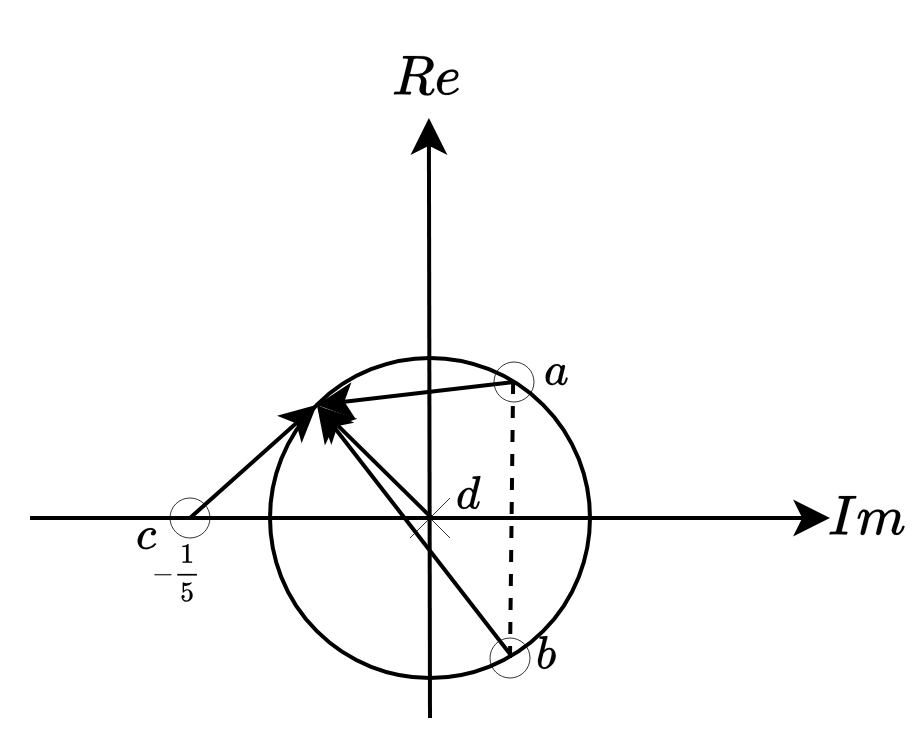
\includegraphics[width=0.5\linewidth]{images/spec1.png}
\end{figure}
In this case we have that the spectral density function is computed as: 
\[\Gamma_y(\omega)=\dfrac{\left\lvert a \right\rvert^2\left\lvert b \right\rvert^2\left\lvert c \right\rvert^2}{\left\lvert d \right\rvert^2}\lambda^2\]

We start in $e^{j0}$, here we have: 
\begin{itemize}
    \item $\left\lvert a \right\rvert^2=1$
    \item $\left\lvert b \right\rvert^2=1$
    \item $\left\lvert c \right\rvert^2=\frac{25}{4}$
    \item $\left\lvert d \right\rvert^2=1$
\end{itemize}
As a result we have that: 
\[\Gamma_y(0)=\dfrac{25}{4}\]


We start in $e^{j\frac{\pi}{2}}$, here we have: 
\begin{itemize}
    \item $\left\lvert a \right\rvert^2=2-\sqrt{3}$
    \item $\left\lvert b \right\rvert^2=2+\sqrt{3}$
    \item $\left\lvert c \right\rvert^2=\frac{13}{4}$
    \item $\left\lvert d \right\rvert^2=1$
\end{itemize}
As a result we have that: 
\[\Gamma_y\left(\frac{\pi}{2}\right)=\dfrac{13}{4}\]

We start in $e^{j\pi}$, here we have: 
\begin{itemize}
    \item $\left\lvert a \right\rvert^2=3$
    \item $\left\lvert b \right\rvert^2=3$
    \item $\left\lvert c \right\rvert^2=\frac{1}{4}$
    \item $\left\lvert d \right\rvert^2=1$
\end{itemize}
As a result we have that: 
\[\Gamma_y\left(\pi\right)=\dfrac{9}{4}\]

Note that 
\[\Gamma_y\left(\frac{\pi}{3}\right)=0\]

Now it is possible to plot the graph. 